If you haven't downloaded and unzipped \href{https://libaoj.in/courses/2021f/MATH3341/zip/Math.3341.zip}{\texttt{Math.3341.zip}}. Download and unzip it under \verb|H:| (H Drive if you are working on the Remote Lab). Change the current working directory by typing \verb|cd H:\Math.3341\Math.3341.Lab.08| in the Command Window, and type \verb|edit lab_08_script| in the Command Window to edit \verb|lab_08_script.m|.

%---------------------------------------------
\section{Polynomial Interpolation Routines}
%---------------------------------------------
\begin{enumerate}[(a)]
    \item Fit \verb|xdata| and \verb|ydata| by an \verb|n|th order polynomial using \verb|polyfit|. Then use \verb|polyval| to evaluate the polynomial at \verb|x|.
    \item Evaluate the cubic spline of \verb|xdata| and \verb|ydata| at \verb|x| using \verb|spline| command.
    \item Now use the \verb|pchip| command to find the values of the piecewise cubic Hermite interpolating polynomial at \verb|x|.
    \item Make a copy of your implementation of Lagrange interpolation for Homework 5. Use your function to find the function values of the Lagrange interpolation polynomial at \verb|x|.
    \item Uncomment ``3 Plot interpolation polynomials" section, which will create the figure comparing each of the polynomial interpolations. If you cannot get your Lagrange interpolation polynomial to work, comment in the relevant lines of code that plot that figure. Expected plot is shown in Figure \ref{fig:1}.
\end{enumerate}
\section{Derivatives of Interpolation Polynomials}
\begin{enumerate}[(a)]
\item \label{enum:II1} Use \verb|polyder| to calculate the coefficients of the first derivative of the interpolation polynomial given by \verb|polyfit| that you constructed, and evaluate it at \verb|x| using \verb|polyval|.
\item Repeat \eqref{enum:II1} to find the second derivative of the interpoation polynomial.
    \item Fit \verb|xdata| and \verb|ydata| using cubic spline and store the structure of the cubic spline interpolation polynomial to \verb|cs_struct|.
    \item Using slicing technique to extract the columns of \verb|cs_struct.coefs| which correspond to each coefficient of the piecewise cubic spline, and store each of these columns in \verb|b|, \verb|c|, \verb|d|, respectively.
    \item Use these coefficients along with \verb|xdata|, \verb|x| to evaluate the first and second derivatives of the spline using \verb|cubic_spline_der.m|. Use \verb|help cubic_spline_der| to get details of the function.
    \item Uncomment ``4 Plot derivatives" section to generate corresponding plots. Expected plot is shown in Figure \ref{fig:2}.
\end{enumerate}

At the end of the day, upload \verb|lab_08_script.m|, \verb|lab_08_figure_01.pdf| and \verb|lab_08_figure_02.pdf| to Overleaf (make sure you change the caption for the figures), then recompile, and submit the generated .pdf file on WyoCourses.

\begin{figure}[!hbtp]
    \centering
    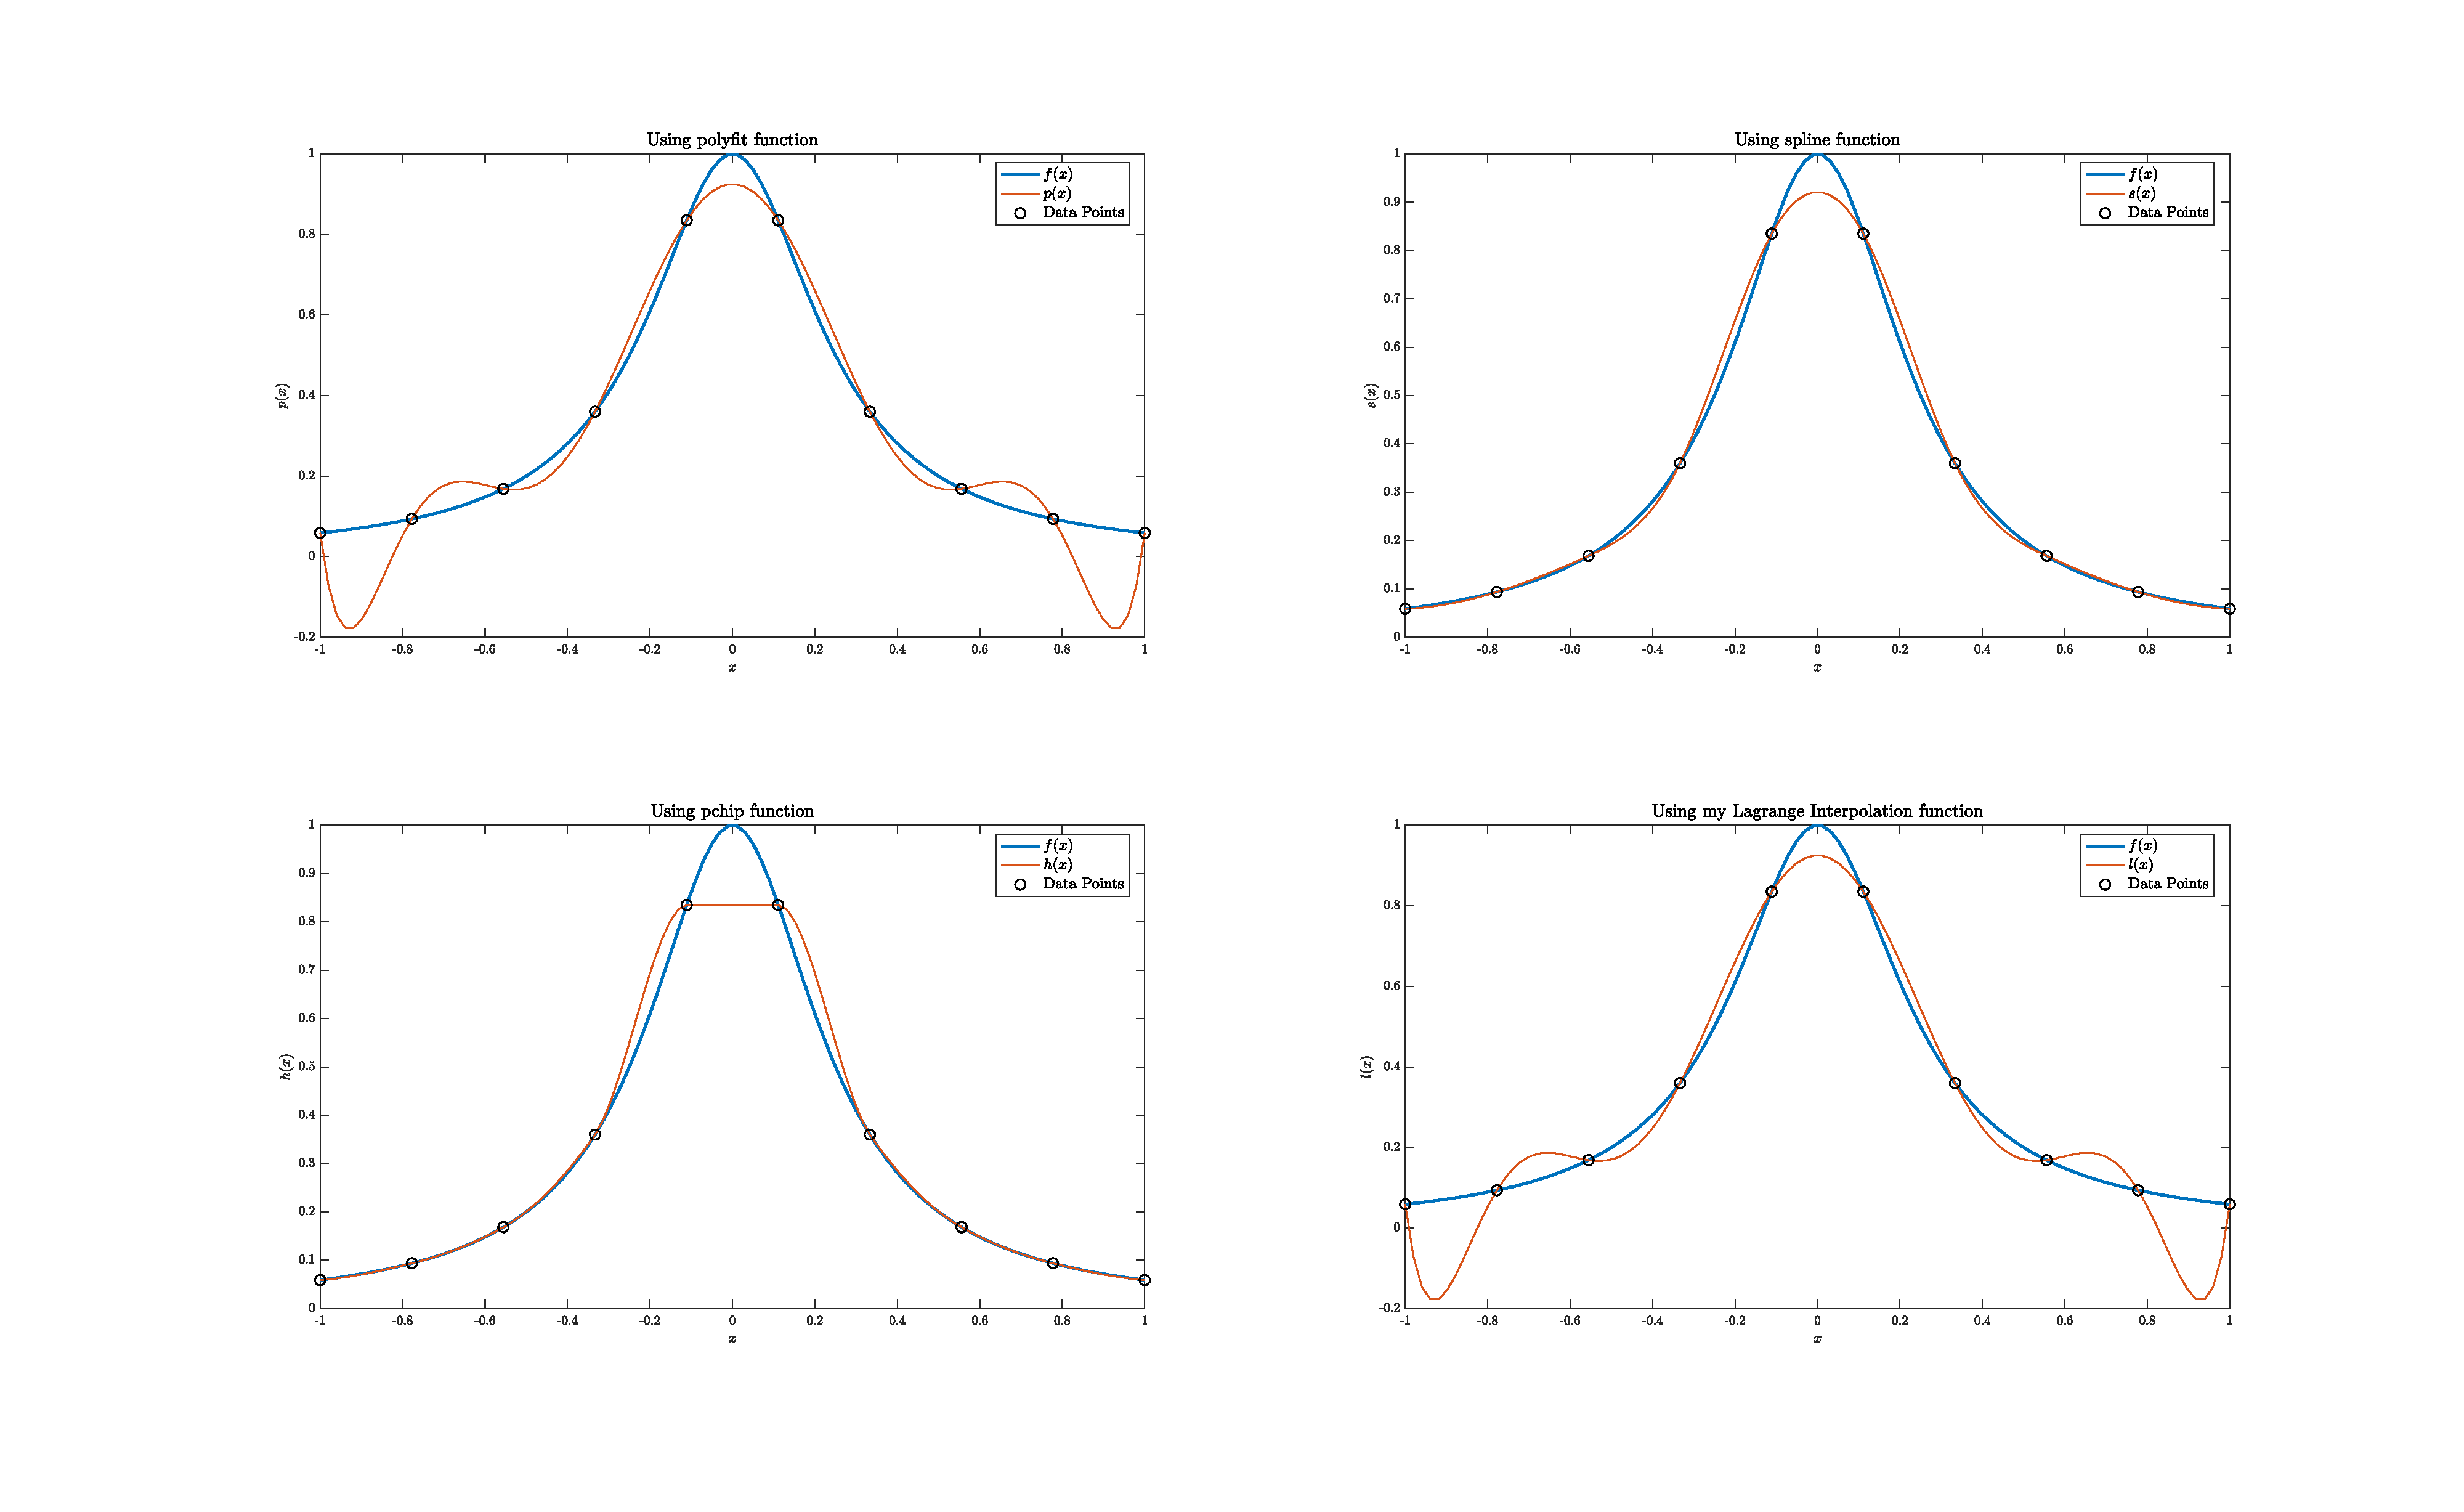
\includegraphics[width=\textwidth]{../Math.3341.Lab.08.ans/lab_08_figure_01.pdf}
    \caption{Polynomial Interpolation using different routines}
    \label{fig:1}
\end{figure}
\begin{figure}[!hbtp]
    \centering
    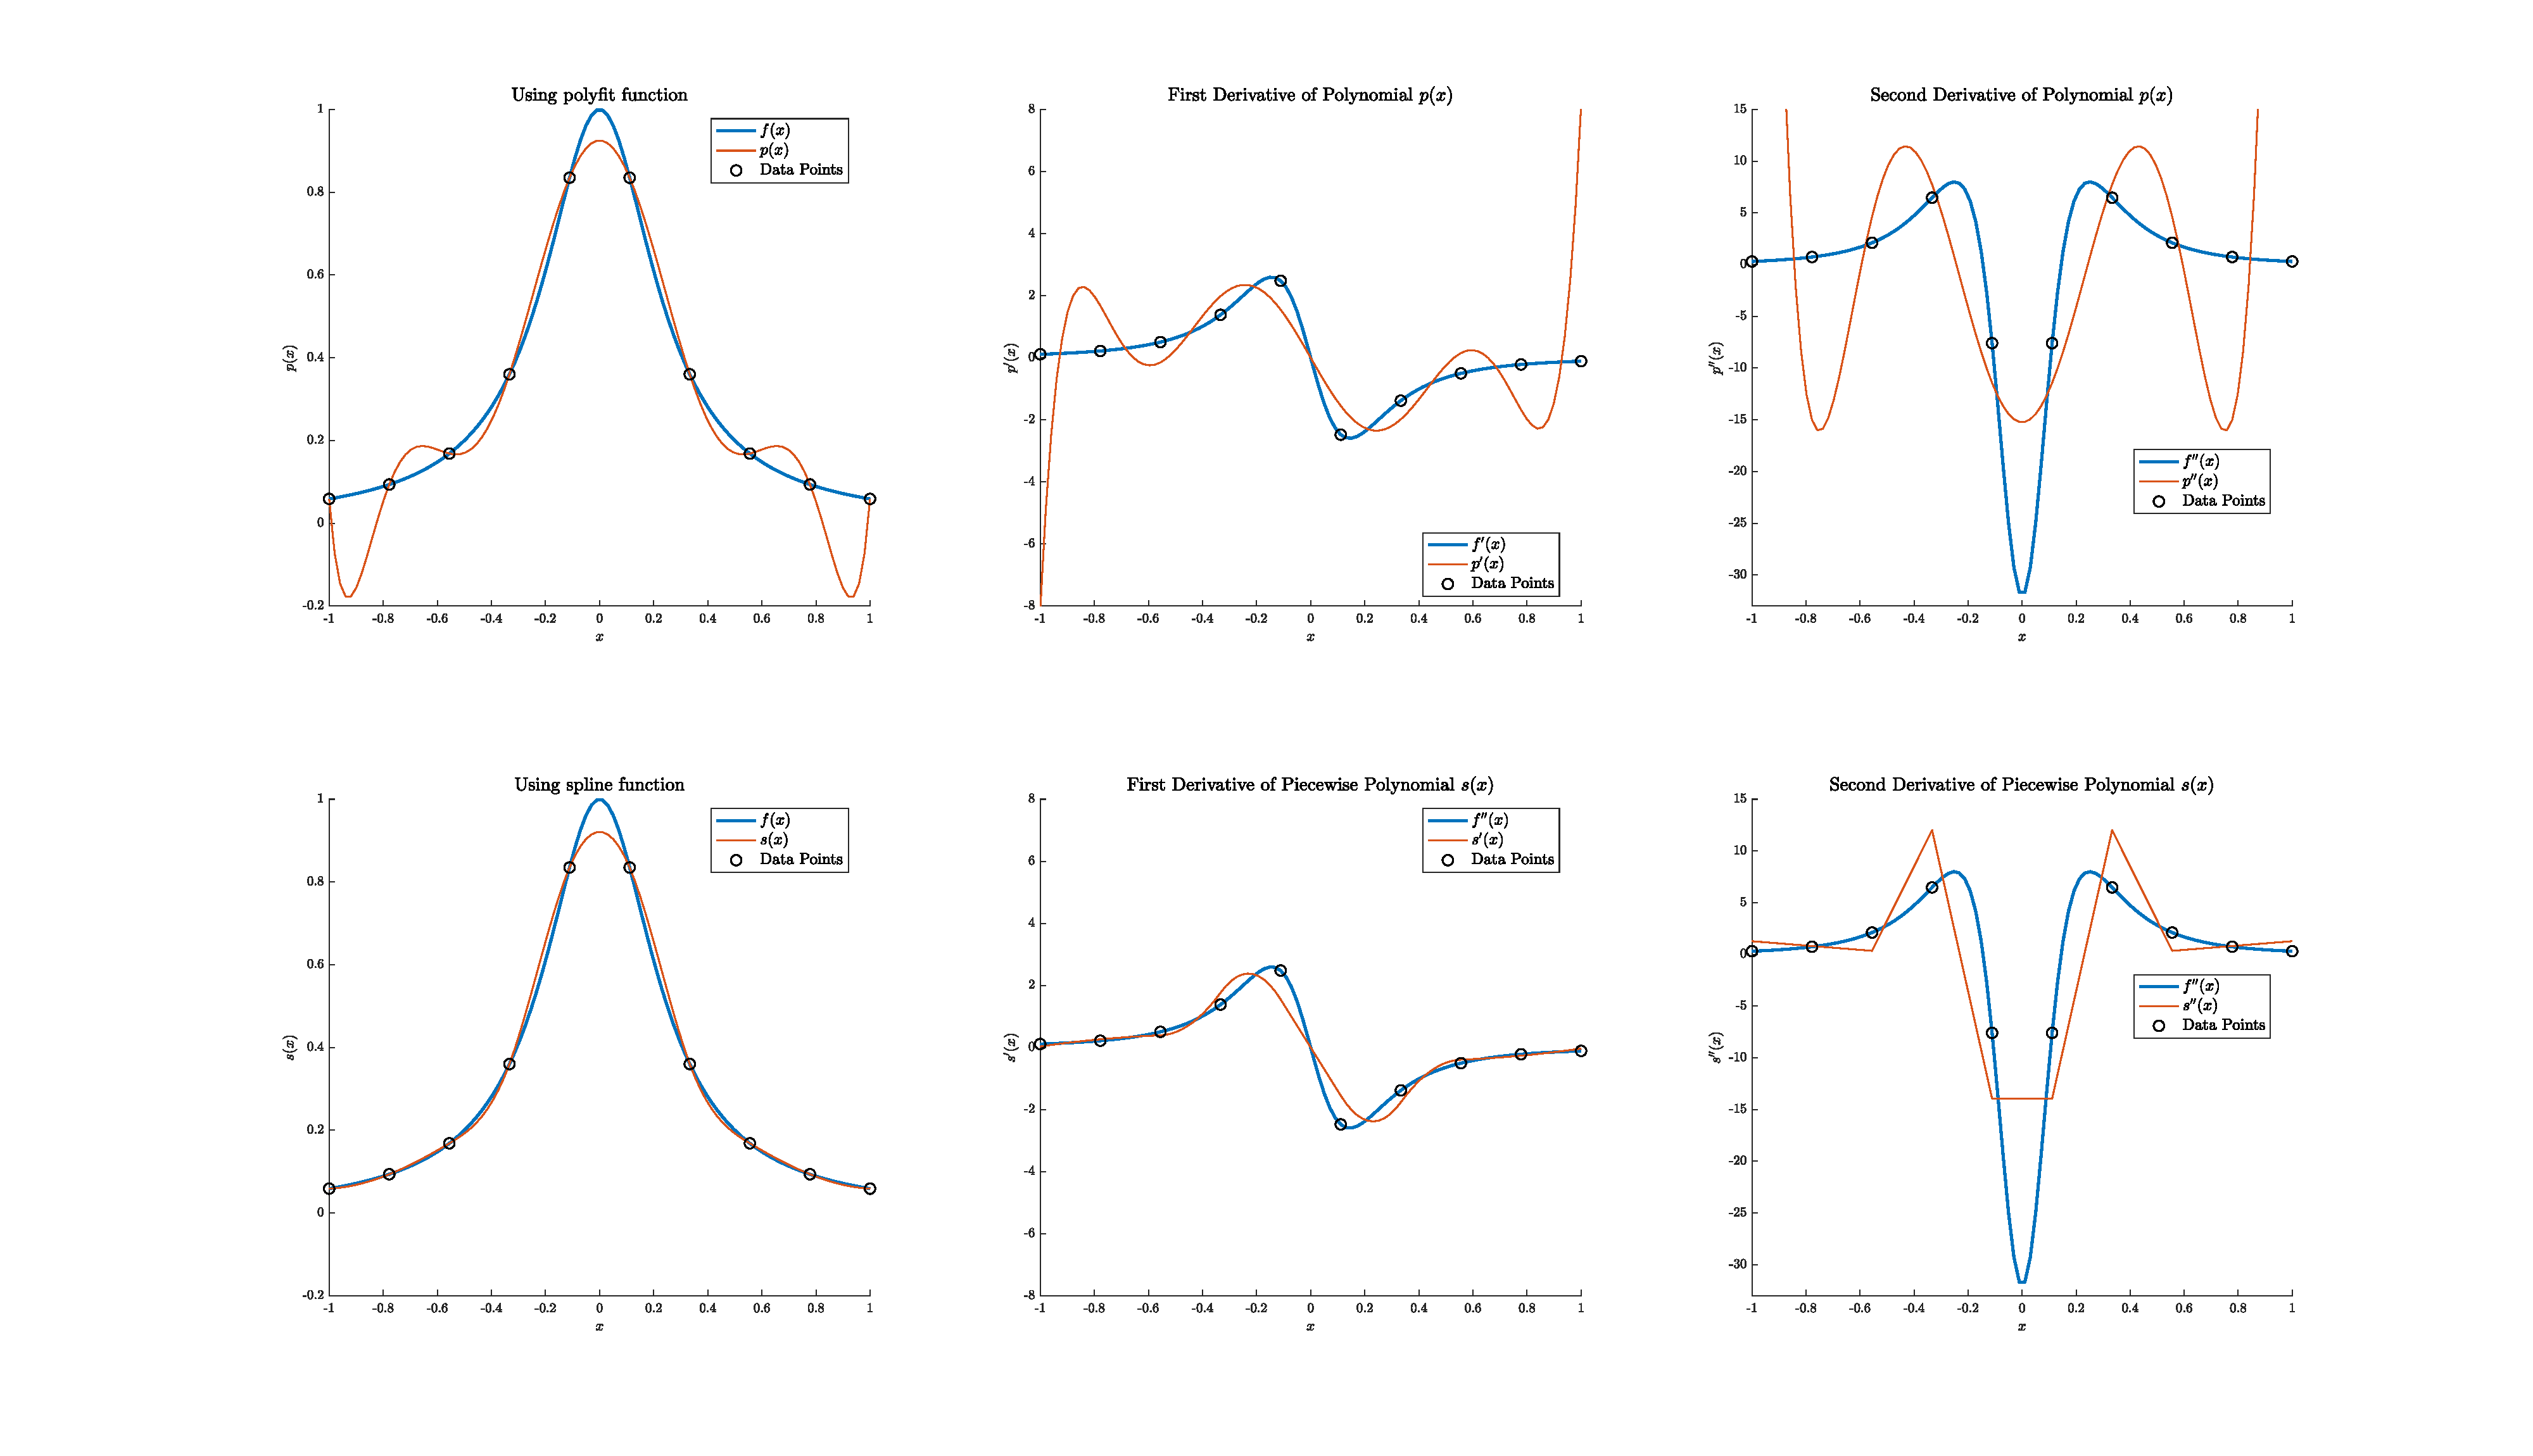
\includegraphics[width=\textwidth]{../Math.3341.Lab.08.ans/lab_08_figure_02.pdf}
    \caption{Derivatives of Interpolation Polynomials}
    \label{fig:2}
\end{figure}
